\section{Cinemática} \label{sec:cinematica}

La cinemática es una rama de la robótica que estudia el movimiento de los robots sin considerar las fuerzas que 
lo generan. Se enfoca en la posición, orientación, 
velocidad y aceleración de los elementos de un robot, a partir de sus articulaciones \cite{Barrientos_fundamentos_robotica}.


Existen dos tipos principales de análisis cinemático:

\begin{itemize}
	\item \textbf{Cinemática directa:} Permite obtener la posición y orientación del efector final a partir de los valores conocidos de las articulaciones.
	\item \textbf{Cinemática inversa:} Determina los valores que deben adoptar las articulaciones para alcanzar una posición y orientación deseada del efector final.
\end{itemize}

Para ver el desarrollo del algoritmo implementado en MATLAB, consultar la \hyperref[sec:proceso_cinematica]{sección del proceso de Cinemática}.



\begin{figure}[h]
	\centering
	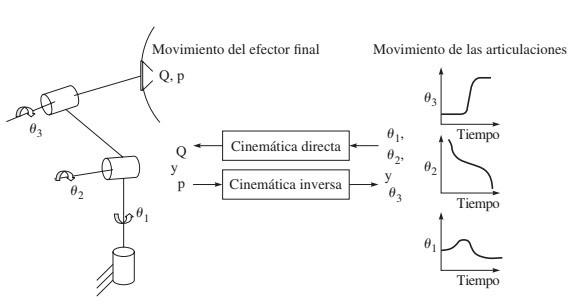
\includegraphics[height=8cm]{Cinematica.jpg}
	\caption{Representación de cinemática directa e inversa \cite{Barrientos_fundamentos_robotica}}
	\label{fig:cinematica-dir-inv}
\end{figure}
\pagebreak[4]  

\subsection{Cinemática Directa}

La cinemática directa se basa en un modelo geométrico del robot. Utiliza parámetros estandarizados como los del método de \textbf{Denavit-Hartenberg (DH)}, que permiten describir la relación espacial entre eslabones consecutivos mediante matrices de transformación homogénea \cite{saha2010}.

La transformación de un sistema de coordenadas \(i-1\) al sistema \(i\) se define mediante:

\[
T_i^{i-1} =
\begin{bmatrix}
	\cos\theta_i & -\sin\theta_i \cos\alpha_i & \sin\theta_i \sin\alpha_i & a_i \cos\theta_i \\
	\sin\theta_i & \cos\theta_i \cos\alpha_i & -\cos\theta_i \sin\alpha_i & a_i \sin\theta_i \\
	0 & \sin\alpha_i & \cos\alpha_i & d_i \\
	0 & 0 & 0 & 1
\end{bmatrix}
\]

El producto secuencial de estas matrices para todos los eslabones permite obtener la transformación total del sistema base hasta el efector final:

\[
T_0^n = T_1^0 \cdot T_2^1 \cdot \ldots \cdot T_n^{n-1}
\]

\subsection{Cinemática Diferencial}

La cinemática diferencial se ocupa de la relación entre la velocidad de las articulaciones y la velocidad lineal y angular del efector final. Esta relación se expresa mediante el \textbf{jacobiano}, una matriz que vincula ambos conjuntos de velocidades \cite{siciliano2010robotics}:

\[
\dot{x} = J(q) \cdot \dot{q}
\]

Donde:
\begin{itemize}
	\item \( \dot{x} \) es el vector de velocidades lineales y angulares del efector final.
	\item \( \dot{q} \) es el vector de velocidades articulares.
	\item \( J(q) \) es la matriz jacobiana, función de las coordenadas articulares \( q \).
\end{itemize}

El jacobiano también es muy importante para detectar y  resolver problemas de cinemática inversa cuando se usan métodos numéricos.

\subsection{Cinemática Inversa}

La cinemática inversa busca determinar los valores articulares necesarios para alcanzar una posición y orientación deseada del efector final. Es un problema más complejo que la cinemática directa, ya que puede tener múltiples soluciones, una única solución, o incluso no tener solución \cite{saha2010}.

Una forma común de resolverlo es mediante métodos iterativos. En este proyecto se implementó un método basado en el uso del gradiente o del jacobiano, que permiten acercarse de manera progresiva a la configuración deseada. El método numérico ajusta los valores de las articulaciones a partir del error entre la posición actual y la deseada, hasta minimizarlo por debajo de un umbral.

Existen diferentes enfoques como el método del descenso del gradiente, el método de Newton-Raphson, la pseudoinversa del jacobiano y otras técnicas avanzadas \cite{siciliano2010robotics}. En nuestro caso, se aplicó la pseudoinversa del jacobiano implementada en MATLAB.
